\documentclass[a4paper,11pt,twocolumn]{article}
\usepackage{fancyhdr}
\usepackage{enumerate}
\usepackage{times}
\usepackage{mathptmx}
\usepackage{amsmath}
\usepackage{amsfonts}
\usepackage{amssymb}
\usepackage{graphicx}
\usepackage[top=2cm, bottom=2cm, left=2cm, right=2cm]{geometry}

\setlength{\columnsep}{7mm}

\newcommand{\homeworkno}{3.10}
\pagestyle{fancy}
\lhead{Problem Solving: Homework \homeworkno}
\chead{}
\rhead{Chen Shaoyuan (161240004)}
\lfoot{}
\cfoot{\thepage}
\rfoot{}

\allowdisplaybreaks[4]
%\renewcommand{\labelenumi}{\textbf{\emph{\alph{enumi}}.}}
\begin{document}
  \title{Problem Solving: Homework \homeworkno}
  \author{Name: Chen Shaoyuan \and Student ID: 161240004}
  \maketitle

  \section{[TJ] Exercise 3-3}
  The Cayley table formed by symmetries of a rectangle is: \par
  \begin{table}[h]
  \begin{tabular}{c|cccc}
    % after \\: \hline or \cline{col1-col2} \cline{col3-col4} ...
    $\circ$ & id & $\rho$ & $\mu_h$ & $\mu_v$ \\ \hline
    id & id & $\rho$ & $\mu_h$ & $\mu_v$ \\
    $\rho$ & $\rho$ & id & $\mu_v$ & $\mu_h$ \\
    $\mu_h$ & $\mu_h$ & $\mu_v$ & id & $\rho$ \\
    $\mu_v$ & $\mu_v$ & $\mu_h$ & $\rho$ & id
  \end{tabular}
  \end{table}
  where $\rho$ denotes $180^\circ$ rotation, $\mu_h, \mu_v$ denote reflection across the horizontal axis and the vertical axis, id denotes identity.
  The Cayley table for $\mathbb{Z}_4$ is: \par
  \begin{table}[h]
  \begin{tabular}{c|cccc}
    % after \\: \hline or \cline{col1-col2} \cline{col3-col4} ...
    $\cdot$ & 0 & 1 & 2 & 3 \\ \hline
    0 & 0 & 1 & 2 & 3 \\
    1 & 1 & 2 & 3 & 0 \\
    2 & 2 & 3 & 0 & 1 \\
    3 & 3 & 0 & 1 & 2
  \end{tabular}
  \end{table}
  There are 4 elements in each group. \par
  The groups are not same, because they contain different elements.

  \section{[TJ] Exercise 3-6}
  The Cayley table for $\mathbb{Z}_4$ is: \par
  \begin{table}[h]
  \begin{tabular}{c|cccc}
    % after \\: \hline or \cline{col1-col2} \cline{col3-col4} ...
    $\cdot$ & 0 & 1 & 2 & 3 \\ \hline
    0 & 0 & 1 & 2 & 3 \\
    1 & 1 & 2 & 3 & 0 \\
    2 & 2 & 3 & 0 & 1 \\
    3 & 3 & 0 & 1 & 2
  \end{tabular}
  \end{table}

  \section{[TJ] Exercise 3-7}
  First, we show that $*$ is a mapping from $S \times S$ to $S$. If $a, b \neq -1$, then $a*b = a+b+ab = (a+1)(b+1)-1 \neq -1$. Hence the closure holds. \par
  Second, the identity is $0$, for every $a \in S$, $0 * a = 0 + a = a$. Likewise $a * 0 = a$. \par
  Third, let's verify the associativity:
  \begin{align*}
    (a*b)*c &= (a + b + ab)*c \\
     &= (a+b+ab) + c + (a+b+ab)c \\
     &= a + b + c + ab + ac + bc + abc \\
     a*(b*c) &= a*(b+c+bc) \\
     &= a + b + c + bc + a(b+c+bc) \\
     &= a + b + c + ab + ac + bc + abc
  \end{align*}
  So the associativity holds.
  Fourth, for every element $a \in S$, the inverse of $a$ is $1/(a+1) - 1$, for
  \begin{align*}
    a*(1/(a+1) - 1) &= a + 1/(a+1) - 1 + a(1/(a+1) - 1) \\
    &= a + 1 - 1 - a \\
    &= 0
  \end{align*}
  Likewise $(1/(a+1)-1)*a = 0$. \par
  Therefore, $(S, *)$ is a group. Also, it is easy to verify that $a * b = b * a$, hence it is also abelian.

  \section{[TJ] Exercise 3-17}
  \begin{align*}
    G_1 &= (\mathbb{Z}_8, +_8) \\
    G_2 &= (\mathbb{Z}_8, \oplus) \\
    G_3 &= (\{e^{2 \pi i / 8} : i \in \mathbb{Z}_8\}, \cdot)
  \end{align*}
  where $+_8$ means plus modulo 8, $\oplus$ means bitwise exclusive-or, $\cdot$ means the multiplication of two complex numbers. \par
  These groups are different, because the sets of elements of the groups are different, or the binary operations differ.

  \section{[TJ] Exercise 3-28}
  \begin{enumerate}
    \item If $m = 0$ or $n = 0$, then the $g^m = e$ or $g^n = e$, so the conclusion holds. If both $m$ and $n$ are positive, note that
        $$ g^n = g^{n-1} g = (g^{n-2} g) g  = g^{n-2} g^2 = \cdots = g g^{n-1} $$
        so
        \begin{align*}
          g^m g^n &= g^m (g g^{n-1}) = (g^m g) g^{n-1} \\ &= g^{m+1} g^{n-1} = \cdots = g^{m+n}
        \end{align*}
        Likewise, when both $m$ and $n$ are negative, the conclusion holds. \par
        When one of $m$ and $n$, assume with out loss of generality, $n$, is positive, and the other is negative, we have
        \begin{align*}
          g^m g^n &= (g^{m+1} g^{-1}) (g g^{n-1}) = g^{m+1} (g^{-1}g)g^{n-1} \\ &= g^{m+1} g^{n-1} = \cdots = g^{m+n}
        \end{align*}
        Therefore, the conclusion holds.
    \item If $n$ is non-negative, then
      $(g^m)^n = (g^m)^{n-1} g^m  = (g^m)^{n-2} g^m g^m = (g^m)^{n-2} (g^{2m}) = \cdots = g^{mn}$. \par
      Otherwise, we have $(g^m)^n = ((g^m)^{-1})^{-n} = (g^{-m})^{-n} = g^{mn}$. \par
      So the conclusion holds.
    \item $(gh)^n = ((gh)^{-1})^{-n} = (h^{-1} g^{-1})^{-n}$ \par
    If $G$ is abelian, then
    \begin{align*}
        (gh)^n &= (gh)^{n-1}(gh) = (gh)^{n-2}(ghgh) \\ &= (gh)^{n-2}(gghh) = (gh)^{n-2}(g^2h^2) \\ &= \cdots = g^nh^n
    \end{align*}
    if $n$ is non-negative, otherwise
    $$(gh)^n = (h^{-1}g^{-1})^{-n} = h^n g^n = g^n h^n$$
    So the conclusion holds.
  \end{enumerate}

  \section{[TJ] Exercise 3-36}
  $H$ is a subset of $\mathbb{Q}^*$, and the identity $1 \in H$. For every $g = 2^{k_1}$, $h = 2^{k_2}$, we have $gh = 2^{k_1 + k_2} \in H$, and $g^{-1} = 2^{-k_1} \in H$, hence $H$ is a subgroup of $\mathbb{Q}^*$.

  \section{[TJ] Exercise 3-38}
  $\mathbb{T}$ is a subset of $\mathbb{C}^*$, and the identity $1 \in \mathbb{T}$. For every $g, h \in \mathbb{T}$, we have $|gh| = 1$ and $|g^{-1}| = 1$, so $gh, g^{-1} \in \mathbb{T}$, hence $\mathbb{T}$ is a subgroup of $\mathbb{C}^*$.

  \section{[TJ] Exercise 3-41}
  $H$ is a subset of $G$, and the identity $0_{2 \times 2} \in H$. For every $A, B \in H$, we have $(A+B)_{11} = (A+B)_{22} = 0$, $-A_{11} = -A_{22} = 0$, so $A+B, -B \in H$, hence $H$ is a subgroup of $G$.

  \section{[TJ] Exercise 3-41}
  $ba = a^4b = (a^3a)b = (ea)b = ab$

  \section{[TJ] Exercise 3-52}
  Let $x = e$, we have $y^2 = y$, therefore $y = e$, so the group $G$ contains only the identity, i.e. $G$ is trivial, and of course $G$ is abelian.

  \section{[TJ] Exercise 4-1}
  \begin{enumerate}[(a)]
    \item False. $U(8) = \{1, 3, 5, 7\}$, while none of them is a generator of $U(8)$.
    \item False. 49 is relatively prime to 60, so it is a generator of $\mathbb{Z}_{60}$, while 49 is not prime.
    \item False. Assume, to the contrary that $\mathbb{Q}$ has a generator $a$, then for all $q \in \mathbb{Q}$, there exists an integer $n$, such that $q = na$. However, if $q = a / 2$, such $n$ does not exist. So $\mathbb{Q}$ is not cyclic.
    \item False. Consider the group $\mathbb{Z}_2 \times \mathbb{Z}_2$ (Klein 4-group), all of its subgroups are cyclic, however, the group itself is not cyclic.
    \item True. If $G$ contains any infinite order element $a$, then $G$ contains infinitely many different subgroups: $\langle a \rangle$, $\langle a^2 \rangle$, $\langle a^3 \rangle$, $\cdots$. Therefore, all elements of $G$ have finite order. Since $G$ contains finite number of subgroups, it contains finitely many cyclic subgroups, each of which is finite. Because every element belongs to at least one cyclic subgroup, the group $G$ is exactly the union of all its cyclic subgraphs, which is still finite.
  \end{enumerate}

  \section{[TJ] Exercise 4-12}
  The trivial group is a cyclic group with exactly one generator. \par
  The cyclic group $\mathbb{Z}$ has exactly two generators, 1 and -1. \par
  The cyclic group $\mathbb{Z}_8$ has exactly four generators, 1, 3, 5 and 7. \par
  For arbitrary $n$, since every cyclic group is isomorphic to either $\mathbb{Z}$ or $\mathbb{Z}_n$, we only have to consider $\mathbb{Z}_n$. So, whether there exists a cyclic group with $n$ generators depends on whether there exists positive integer $m$ such that $\phi(m) = n$, where $\phi$ is the Euler $\phi$-function. For example, $\phi(3) = 2$, so $\mathbb{Z}_3$ has 2 generators. However, it can be proved in number theory that there does not exist positive integer $m$ such that $\phi(m) = 3$, hence there does not exist cyclic group that contains exactly 3 generators.

  \section{[TJ] Exercise 4-21}
  The 5th roots of unity are: $1$, $e^{2\pi i/5}$, $e^{4\pi i/5}$, $e^{6\pi i/5}$, $e^{8\pi i/5}$. \par
  \begin{figure}[h]
    \centering
    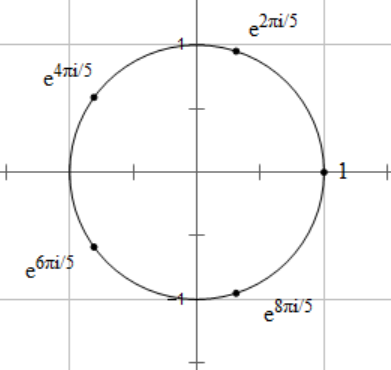
\includegraphics{root5.png}
  \end{figure}
  The generators of this group are $e^{2\pi i/5}$, $e^{4\pi i/5}$, $e^{6\pi i/5}$, $e^{8\pi i/5}$. \par
  The primitive 5-th roots of unity are $e^{2\pi i/5}$, $e^{4\pi i/5}$, $e^{6\pi i/5}$, $e^{8\pi i/5}$.

  \section{[TJ] Exercise 4-24}
  $\mathbb{Z}_{pq}$ has $\phi(pq)$ generators, since $p$ and $q$ are distinct primes, we have $\phi(pq) = \phi(p)\phi(q) = (p-1)(q-1)$, because $\phi$ is a multiplicative function. So $\mathbb{Z}_{pq}$ has $(p-1)(q-1)$ generators.

  \section{[TJ] Exercise 4-32}
  The order of $y$ is $n/\gcd(k, n) = n$, which means $\langle y \rangle$ contains as many elements as $G$ has, i.e. $y$ is a generator of $G$.

  \section{[TJ] Exercise 5-3}
  \begin{enumerate}[(a)]
    \item (16)(15)(13)(14), even
    \item (16)(15)(24)(23), even
    \item (16)(12)(14)(12)(14), odd
    \item (14)(15)(12)(17)(13)(12)(14)(12)(13)(16)(14)(15), even
    \item (17)(13)(16)(12)(14), odd
  \end{enumerate}

  \section{[TJ] Exercise 5-5}
  The subgroups of $S_4$ are
  \begin{itemize}
    \item trivial subgroups: $\{\text{id}\}$;
    \item subgroups of order 2: $\{\text{id}, (12)\}$, $\{\text{id}, (13)\}$, $\{\text{id}, (14)\}$, $\{\text{id}, (23)\}$, $\{\text{id}, (24)\}$, $\{\text{id}, (34)\}$, $\{\text{id}, (12)(34)\}$, $\{\text{id}, (13)(24)\}$, $\{\text{id}, (14)(23)\}$;
    \item cyclic subgroups of order 3: $\langle (123) \rangle$, $\langle (124) \rangle$, $\langle (134) \rangle$ and $\langle (234) \rangle$;
    \item cyclic subgroups of order 4: $\langle (1234) \rangle$, $\langle (1324) \rangle$, $\langle (1243) \rangle$;
    \item Klein 4-groups: \{\text{id}, (12), (34), (12)(34)\},
        \{\text{id}, (13), (24), (13)(24)\},
        \{\text{id}, (14), (23), (14)(23)\},
        \{\text{id}, (12)(34), (13)(24), (14)(23)\};
    \item $S_3$ subgroups: permutations of $\{1, 2, 3\}$, $\{1, 2, 4\}$, $\{1, 3, 4\}$ and $\{2, 3, 4\}$;
    \item ``rectangle'' subgroups: $\{\text{id}, (13), (24),\\ (13)(24), (12)(34), (14)(23), (1234), (1432)\}$, $\{\text{id}, (14), (23), (14)(23), (12)(34), (13)(24), \\ (1243), (1342)\}$ and $\{\text{id}, (12), (34), (14)(23), \\ (12)(34), (13)(24), (1324), (1423)\}$;
    \item the alternating group: $A_4$;
    \item $S_4$ itself.
  \end{itemize}
  The sets are
  \begin{enumerate}[(a)]
    \item $\{\sigma \in S_4 : \sigma(1) = 3\} = \{(13), (13)(24), \\ (132), (134), (1324), (1342)\}$;
    \item $\{\sigma \in S_4 : \sigma(2) = 2\} = \{\text{id}, (13), (14), (34), \\ (134), (143)\}$;
    \item $\{\sigma \in S_4 : \sigma(1) = 3 \text{ and } \sigma(2) = 2\} =  \{(13), \\ (134)\}$;
  \end{enumerate}

  \section{[TJ] Exercise 5-16}
  Let 1, 2, 3, 4 denote the four vertices of a tetrahedron, respectively. Then all its rigid motions can be represented as a permutation of 1, 2, 3, 4, and they are:
  \begin{itemize}
    \item eight $60^\circ$ rotation operations: (123), (321), (124), (421), (134), (431), (234), (432);
    \item three $120^\circ$ rotation operations: (12)(34), (13)(24), (14)(23);
    \item and, the identity: id.
  \end{itemize}
  Note that these permutations are exactly all even permutations on 4 letters, so it is the same as $A_4$.

  \section{[TJ] Exercise 5-27}
  We only have to prove that $\lambda_g$ is one-to-one and onto. \par
  For every $b \in G$, there exists $a = g^{-1}b$, such that
  $$ \lambda_g(a) = gg^{-1}b = b$$
  so $\lambda_g$ is onto. \par
  For every $a, b \in G$, if $\lambda_g(a) = \lambda_g(b)$, i.e. $ga = gb$, then we have $a = b$, so $\lambda_g$ is one-to-one. \par
  Therefore, $\lambda_g$ is one-to-one and onto, so $\lambda_g$ is a permutation of $G$.

  \section{[TJ] Exercise 5-29}
  The centers of $D_8$, $D_10$ are $\{\text{id}, i\}$, where $i$ denotes inversion through the center of the polygon. \par
  For arbitrary $n$, the center of $D_n$ is $\{\text{id}\}$ if $n$ is odd, or $\{\text{id}, i\}$ is even. Note, that only when $n$ is even $D_n$ contains $i$. \par
  It is obvious that id and $i$ are central. For any element other than id, it is either a reflection or a rotation. Let $\rho$ be any rotation and $\mu$ be any reflection. It is easy to verify that $\rho \mu = \mu \rho^{-1}$. Note that $\rho^{-1} = \rho$ if and only if $\rho = i$. So any element other than id and $i$ is not central.

  \section{[TJ] Exercise 6-11}
  (a) $\rightarrow$ (b): for every $h \in H$, there exists $h' \in H$, such that $g_1h = g_2h'$. Hence we have $hg_2^{-1} = h(g_1hh'^{-1})^{-1} = (hh'^{-1}h^{-1})g_1^{-1} \in Hg_1^{-1}$, so $Hg_2^{-1} \subseteq Hg_1^{-1}$. Likewise we have $Hg_1^{-1} \subseteq Hg_2^{-1}$, so $Hg_1^{-1} = Hg_2^{-1}$. \par
  (b) $\rightarrow$ (a): for every $h \in H$, there exists $h' \in H$, such that $hg_1^{-1} = h'g_2^{-1}$. Hence we have $g_2h = (g_1h^{-1}h')h = g_1(h^{-1}h'h) \in g_1H $, so $g_2H \subseteq g_1H$. Likewise $g_1H \subseteq g_2H$, so $g_1H = g_2H$. \par
  (a) $\rightarrow$ (c) is immediate. (also we have $g_2H \subseteq g_1H$) \par
  (c) $\rightarrow$ (d): $g_2H \subseteq g_1H$, and $g_2 = g_2e$ is an element of the former one, so it is also an element of the latter one, i.e. $g_2 \in g_1H$. \par
  (d) $\rightarrow$ (e): since $g_2 \in g_1 H$, there exists $h \in H$, such that $g_2 = g_1h$, so $g_1^{-1}g_2 = h \in H$. \par
  (e) $\rightarrow$ (a): for every $h \in H$, we have
  $ g_1h = g_1(g_1^{-1}g_2)(g_1^{-1}g_2)^{-1}h = g_2((g _1^{-1}g_2)^{-1}h) \in g_2H$ and $g_2h = g_2(g_1^{-1}g_2)^{-1}(g_1^{-1}g_2)h = g_1(g_1^{-1}g_2h) \in g_1 H$, so every element of $g_1 H$ is an element of $g_2H$, and vice versa. Hence $g_1H = g_2H$. \par
  Therefore, these 5 conditions are equivalent.

  \section{[TJ] Exercise 6-12}
  Consider the left coset $gH$ and right coset $Hg$ for arbitrary $g \in G$. For every $h \in H$, $gh = gh(g^{-1}g) = (ghg^{-1})g \in Hg$, which means $gH \subseteq Hg$; $hg = (gg^{-1})hg = g(g^{-1}h(g^{-1})^{-1}) \in gH$, which means $Hg \subseteq gH$, so $gH = Hg$. Therefore, the right cosets are identical to left cosets.

  \section{[TJ] Exercise 6-16}
  Since $G$ is finite, every element of $G$ has finite order. Let's consider the elements whose orders are not 2. $G$ contains exactly one element of order 1, the identity. For every $a \in G$ that the order or $a$ are greater than 2, $a^{-1}$ is also an element whose order is greater than 2. Furthermore, $a^{-1} \neq a$, for otherwise $a^2 = 1$, which leads to contradiction. This means that the elements whose orders are greater than 2 can be paired up. Therefore, the number of elements of order 2 is odd. \par
  The conclusion above shows that $G$ contains at least one element of order 2. The cyclic graph generated by such an element is a subgroup of $G$ of order 2.

  \section{[TJ] Exercise 6-21}
  For arbitrary element $a \in G$ ($a \neq e$), the order of $a$ is $p^k$, where $0 < k \leq n$. Then, $a^{p^{k-1}}$ is an element of order $p$, which means $\langle a^{p^{k-1}} \rangle$ is a proper subgroup of order $p$. \par
  If $n \geq 3$, it is true that $G$ must have proper subgroup of order $p^2$. If there exists some element $a$ of order $p^k$, by first Sylow theorem.

  \section{[TJ] Exercise 9-6}
  Suppose $f: \{{\omega_n}^i\} \rightarrow \mathbb{Z}_n$ is defined as
   $$ f({\omega_n}^i) = i $$
  then $f$ is one-to-one and onto. And we have
  \begin{align*}
    & f({\omega_n}^i \cdot {\omega_n}^j) = f({\omega_n}^{(i+j) \bmod n}) = (i+j) \bmod n \\
   =& [f({\omega_n}^i) + f({\omega_n}^j)] \bmod n = (i + j) \bmod n
  \end{align*}
  So the $n$th roots of unity are isomorphic to $\mathbb{Z}_n$.

  \section{[TJ] Exercise 9-7}
  Let $\langle a \rangle = \{e, a, a^2, \cdots, a^{n-1}\}$ denote the cyclic group of order $n$. Suppose $f: \langle a \rangle \rightarrow \mathbb{Z}_n$ is defined as
  $$ f(a^n) = n $$
  then $f$ is one-to-one and onto. And we have
  \begin{align*}
    & f(a^i \cdot a^j) = f(a^{(i+j) \bmod n}) = (i+j) \bmod n\\
   =& [f(a^i) + f(a^j)] \bmod n = (i + j) \bmod n
  \end{align*}
  So $\langle a \rangle$ is isomorphic to $\mathbb{Z}_n$.

  \section{[TJ] Exercise 9-8}
  Suppose, to the contrary, that $\mathbb{Q}$ is isomorphic to $\mathbb{Z}$. Since $\mathbb{Z}$ is cyclic, $\mathbb{Q}$ is also cyclic. However, we have already proved in Exercise 4-1(c) that $\mathbb{Q}$ is not cyclic, which leads to contradiction.

  \section{[TJ] Exercise 9-9}
  We have proved in Exercise 3-7 that $G$ is a group. \par
  We define a map $f$ from $G$ to $\mathbb{R}^*$ as
  $$ f(a) = a + 1 $$
  then $f$ is one-to-one and onto. Also, we have
  \begin{align*}
    & f(a * b) = f(a + b + ab) = a+b+ab+1 \\
    =& f(a)f(b) = (a+1)(b+1) = a+b+ab+1
  \end{align*}
  so $(G, *)$ is isomorphic to $\mathbb{R}^*$.
\end{document}
